\documentclass{article}

\usepackage{amsmath}
\usepackage{amssymb}
\usepackage{hyperref}
\usepackage{url}
\usepackage{graphicx}
\usepackage{geometry}
\usepackage{enumitem}
\usepackage{parskip}
\usepackage{chemfig}
\usepackage{pdfpages}
\usepackage{xcolor}
\usepackage{tikz}
\usepackage{fancybox}
\usepackage{makecell}
\usepackage{pgfplots}
\usepackage{soul}
\usepackage{ulem}
\usepackage{wrapfig}
\usepackage{subcaption}
\usepackage[T1]{fontenc}
\usepackage{esvect}
\usepackage{multirow}
\usepackage{booktabs}
\usepackage{float}
\usepackage{tocloft}
\usepackage{caption}
\usepackage{colortbl}
\usepackage{siunitx}
\usetikzlibrary{arrows}
\usetikzlibrary{decorations.pathreplacing}
\pgfplotsset{compat=1.17}
\usepgfplotslibrary{statistics}
\definecolor{darkgray}{rgb}{0.2, 0.2, 0.2}

% === BIBLIOGRAPHY ===
\usepackage[utf8]{inputenc}
\usepackage{csquotes}
\usepackage[style=apa, backend=biber, doi=true, url=true]{biblatex}
\addbibresource{ref.bib}
\DeclareFieldFormat[article]{volume}{\textbf{#1}}
\DeclareFieldFormat[article]{journaltitle}{\textit{#1}}
% ====================
 
\geometry{
    a4paper,
    total={170mm, 257mm},
    left=20mm,
    top=20mm
}

\hypersetup{
    colorlinks=true,
    linkcolor=black,
    urlcolor=blue,
    pdftitle={Report SW10 - EnCheBio}
}

\newcommand{\figbox}[1]{ 
    \begin{figure*}[ht!]        
        \begin{center}            
            \fbox{#1}        
        \end{center}    
    \end{figure*}
}

\newcommand{\wrapfill}{
    \par
    \ifnum \value{WF@wrappedlines} > 0
        \addtocounter{WF@wrappedlines}{-1}%
        \null\vspace{
            \arabic{WF@wrappedlines}
            \baselineskip
        }
        \WFclear
    \fi
    \phantom{}
}

\newcommand{\cfig}[3]{
    \centering
    \chemfig{#1}
    \captionof{figure}{#3}
    \label{#2}
}


% === LIST OF EQUATIONS ===
\newcounter{myequation}
\renewcommand{\themyequation}{\arabic{myequation}}

\newlistof{myequations}{loe}{\Large List of Equations}
\newcommand{\addequationtotoc}[1]{\addcontentsline{loe}{myequations}{\protect\numberline{\themyequation}#1}}

\renewcommand{\cftmyequationspresnum}{}
\renewcommand{\cftmyequationsaftersnum}{\hspace{1em}}
\setlength{\cftmyequationsnumwidth}{2em}
\cftsetindents{myequations}{1.5em}{2.3em}

\newcommand{\capeq}[3]{
    \refstepcounter{myequation}
    \begin{equation*}
        #1
    \end{equation*}
    \label{#2}
    \begin{center}
        \vspace*{-.4cm}
        \noindent{Equation \themyequation:} #3
    \end{center}
    \addequationtotoc{#3}
}

\newcommand{\refeq}[1]{\hyperref[#1]{[Equation~\ref*{#1}]}}
% =========================

\newcommand{\difference}{\,\backslash\,}
\newcommand{\rem}{\underline{Remark}: }
\newcommand{\nots}{\underline{Notation}: }
\newcommand{\prf}{\underline{Proof}: }
\newcommand{\exs}{\underline{Example}: }
\newcommand{\defs}{\underline{Definition}: }
\newcommand{\wrn}{\underline{Warning}: }
\newcommand{\sht}{\ |\ }
\newcommand{\pph}[1]{\paragraph{#1}\phantom{}\\}

% === TEXT ===
\begin{document}

\hypersetup{citecolor=black}

\begin{minipage}{0.7\textwidth}
    \vspace*{-.8cm} \hspace*{-0.3cm}
    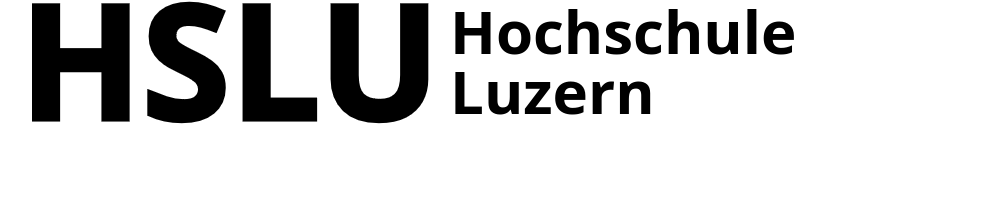
\includegraphics[width=.5\textwidth]{media/hslu-logo.png}
\end{minipage}

\vspace*{2cm}

\textbf{\huge Practical 3:}\\[.75cm]
\begin{center}
    \textbf{\huge Analysis of PAHs in Plastics}
    
    \textbf{\huge by GC-MS}\\[1cm]
    
    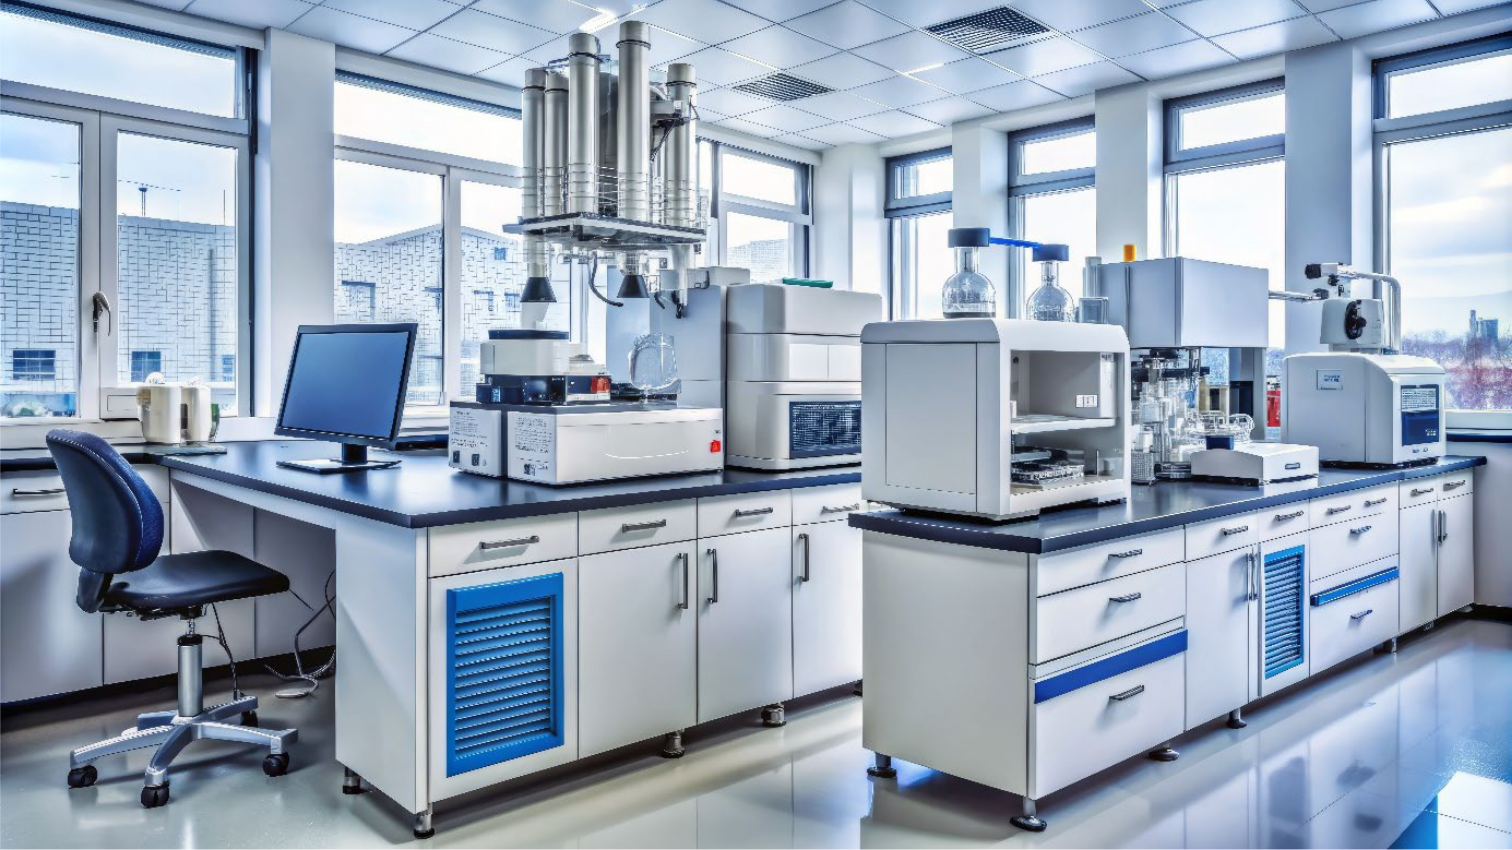
\includegraphics[width=\textwidth]{media/front_practical3.png}\\
\end{center}

\vfill

\setlength{\intextsep}{0pt}%
\begin{wrapfigure}{r}{\textwidth}
    \textbf{\Large Environmental Chemistry and Biology HS2024\\[.5cm]
    \large Dr. Macarena San Martín Ruiz\\
    Lecturer}
    \vspace{-2.1cm}
\end{wrapfigure}

\phantom{}\\[-1cm]

\begin{flushright}
        \large
        \textbf{Team 4}\\
        Matteo Frongillo\\
        Ramadhan Nura\\
        Folagbade Popoola\\
        Jonathan Lawrence Boms\\
        Kron Xhemajli
\end{flushright}
\wrapfill
\newpage
\tableofcontents
\pagebreak

\section{Introduction}
The purpose of this experiment is to understand the analysis and quantification of polycyclic aromatic hydrocarbons (PAHs) in plastics using Gas Chromatography-Mass Spectrometry (GC-MS). This involves learning key concepts such as chromatographic separation, detection techniques, and calibration methods.

\section{Materials and Methods}
\subsection{Materials}
\begin{itemize}
    \item Gas chromatograph -- Mass spectrometer
    \item Helium (carrier gas)
    \item Standard PAH kit
    \item Chloroform (solvent)
    \item Vials
    \item Pipettes
\end{itemize}

\subsection{Experimental Procedure}
\subsection{Preparation of diluted solutions for a calibration curve}
\subsubsection{Legend}
\begin{itemize}
    \item $\mathbf{C_i}$: Initial stock concentration ($\mu$g/mL)
    \item $\mathbf{C_t}$: Target concentration ($\mu$g/mL)
    \item $\mathbf{V_s}$: Volume of stock solution required (mL)
    \item $\mathbf{V_t}$: Target volume (mL)
    \item $\mathbf{V_c}$: Volume of chloroform required (mL)
\end{itemize}

\subsubsection{Formulas}
\begin{itemize}
    \item Amount of volume of stock solution required $\mathbf{V_s}$:
    \capeq{V_s = \frac{C_t \cdot V_t}{C_i}}{eq:vol_stock}{Stock solution volume}
    \item Volume of chloroform required $\mathbf{V_c}$:
    \capeq{V_c = V_t - V_s}{eq:vol_solvent}{Solvent volume}
\end{itemize}

\subsubsection{Ratios}
\begin{table}[H]
    \centering
    \caption{Diluted solution ratios}
    \begin{tabular}{@{}lcllcl@{}}
        \toprule
        \textbf{Dilution} & $\mathbf{C_i}$ & $\mathbf{C_t}$ & $\mathbf{V_s}$ & $\mathbf{V_t}$ & $\mathbf{V_c}$\\
        \midrule
        1:10 & 10 & 1 & 0.1 & 1 & 0.9\\
        1:100 & 10 & 0.1 & 0.01 & 1 & 0.99\\
        1:1000 & 10 & 0.01 & 0.001 & 1 & 0.999\\
        \bottomrule
    \end{tabular}
    \label{tab:ratios}
\end{table}

\section{Results}
\subsection{PAHs detected}
\subsubsection{LMW PAHs}

\noindent
\begin{minipage}{0.32\textwidth}
\cfig{[:0]*6(=-*6(-=-=-)=-=-)}{ch:naphtalene}{Naphtalene}
\end{minipage}%
\begin{minipage}{0.32\textwidth}
\cfig{[:0]*6(=-*6(-=-=(-[:112]-[:180]-[:249 ])-)=-=-)}{ch:acenaphthene}{Acenaphthene}
\end{minipage}%
\begin{minipage}{0.32\textwidth}
\cfig{[:0]*6(=-*6(-=-=(-[:112]=[:180]-[:249 ])-)=-=-)}{ch:acenaphthylene}{Acenaphthylene}
\end{minipage}

\vspace{0.5cm}

\noindent
\begin{minipage}{0.32\textwidth}
\cfig{*6(=-(*5(-(*6(-=-=-=))----))=-=-)}{ch:fluorene}{Fluorene}
\end{minipage}%
\begin{minipage}{0.32\textwidth}
\cfig{*6(=-(*6(-(*6(-=-=--))=-=-))=-=-)}{ch:phenanthrene}{Phenanthrene}
\end{minipage}%
\begin{minipage}{0.32\textwidth}
\cfig{*6(=-(*6(-=(*6(-=-=--))-=--))=-=-)}{ch:anthracene}{Anthracene}
\end{minipage}

\subsubsection{HMW PAHs}

\noindent
\begin{minipage}{0.32\textwidth}
\cfig{*6(-=(*6(-=-(*6(-(*6(-=-=--))=-=--))=--))-=-=)}{ch:chrysene}{Chrysene}
\end{minipage}%
\begin{minipage}{0.32\textwidth}
\cfig{*6(-=(*6(-=-=(-[:112]([:120]*6(-=-=-=))-[:180]-[:249])--))-=-=)}{ch:fluoranthene}{Fluoranthene}
\end{minipage}%
\begin{minipage}{0.32\textwidth}
\cfig{*6(=-(*6(-=-=--))=(*6(--=---))-(*6(=-=-=-))--)}{ch:pyrene}{Pyrene}
\end{minipage}

\subsubsection{Data sheet}
\begin{table}[H]
    \centering
    \caption{Compounds data}
    \begin{tabular}{@{}llllll@{}}
        \toprule
        \textbf{Nr.} & \textbf{Compound} & \textbf{Concentration} & \textbf{Retention} & \textbf{Peak area} & \textbf{m/z}\\
        & \textbf{name} & \textbf{(ng/mL)} & \textbf{time} & & \textbf{fragments}\\
        \midrule
        1 & \nameref{ch:naphtalene} &  & 4.62 & 938975 & 128\\
        2 & \nameref{ch:acenaphthylene} &  & 7.78 & 1093694 & 152\\
        3 & \nameref{ch:acenaphthene} &  & 8.18 & 1306917 & 154\\
        4 & \nameref{ch:fluorene} &  & 9.35 & 1134899 & 166\\
        5 & \nameref{ch:anthracene} &  & 11.58 & 1115451 & 178\\
        6 & \nameref{ch:phenanthrene} &  & 11.71 & N.D. & 178\\
        7 & \nameref{ch:pyrene} &  & 14.46 & 1358324 & 202\\
        8 & \nameref{ch:fluoranthene} &  & 15.00 & 1533223 & 202\\
        9 & \nameref{ch:chrysene} (1) &  & 18.08 & 133907 & 114\\
        10 & \nameref{ch:chrysene} (2) &  & 18.21 & 992122 & 228\\
        \bottomrule
    \end{tabular}
    \label{tab:calibration-data}
\end{table}

\subsection{Chromatograms}
Include chromatograms here with appropriate annotations.

\subsection{Unknown Sample Analysis}
The peak area for the unknown sample was 300. Using the calibration curve equation, the concentration is determined as:
\capeq{C = \frac{(300 - 0)}{12} = 25\, \text{ng/mL}}{eq:concentration}{Concentration of Chrysene in the unknown sample}

\section{Discussion}
\begin{itemize}
    \item Discuss the separation efficiency, retention times, and peak identification.
    \item Answer questions on compound appearance order, fragmentation, and hydrophobicity.
    \item Explain the differences between the calibration curve method and the internal standard method.
\end{itemize}

\section{Conclusion}
This experiment provided a hands-on understanding of GC-MS analysis for PAHs, highlighting the importance of calibration and method validation for accurate quantification.

\newpage
\listoffigures

\listoftables

\listofmyequations

\printbibliography

\end{document}